%\chapter{Preliminares. } % (fold)

En este capítulo se pretende establecer mediante un análisis, la comparativa realizada entre sistemas o prototipos existentes que hacen uso de herramientas criptográficas para proveer un servicio similar al protocolo criptográfico que se propone en este trabajo terminal. Dicho análisis contendrá detalladamente aquellos elementos técnicos que tienen relación con la criptografía y de qué manera se están utilizando. De igual forma, el capítulo contiene la explicación y el funcionamiento del protocolo criptográfico Dupless, dicho protocolo es la base de la investigación, de la cual surge el desarrollo del protocolo criptográfico que se presenta para este trabajo terminal. 






\section{Estado del Arte. }

Una solución para tener privacidad y evitar duplicación es el $cifrado convergente$ que la proporcionó John R. Douceur, la cual dice que teniendo a $M$ que será el contenido de un archivo de aquí en adelante denominado el mensaje, el cliente primero calcula una clave $K ← H(M)$ mediante la aplicación de una función de hash criptográfica $H$ al mensaje y luego calcula el texto cifrado $C ← E(K, M)$ a través de un esquema de cifrado simétrico determinista. El derivado del mensaje $K$ se almacena por separado cifrándolo con una llave por cliente. Un segundo cliente $B$ cifra el mismo archivo $M$ que producirá el mismo $C$, evitando la duplicación ~\cite{donceur}. Existen sistemas que aplican esta herramienta de cifrado para proteger la información, a continuación, se presenta una tabla comparativa de algunos de estos. \\


%El cifrado convergente consiste en una solución que ocupan los sistemas que se muestran abajo, esta solución pretende dar seguridad y evitar duplicados, esta consiste en que si un usuario quiere subir un archivo para generar su llave debe calcular el hash de dicho archivo, el resultado será su llave para poder cifrarlo, así de esta manera si otro usuario quiere subir el mismo archivo obtendrá la misma llave y así el resultado de los archivos cifrados será el mismo y se podrá evitar así el duplicado en la nube. Pero tiene un problema importante en la parte de la seguridad, ya que no es resistente a ataques por fuerza bruta, esto quiere decir que, si un usuario quiere robar un archivo, para poder descifrarlo necesita el hash del mensaje que se cifro, pero este lo puede obtener realizando varias pruebas con archivos diferentes hasta encontrar un archivo que dé el mismo hash y entonces poder descifrar el archivo correctamente.


\begin{tabular}{ |p{8cm}|p{8cm}| }
\hline
{ \textbf{TahoeFS}} & {\textbf{ABS: The Apportioned Backup System} } \\
\hline
{Firmas Digitales} & {Firmas Digitales} \\
\hline
{SHA256} & {SHA256} \\
\hline
{AES-128} & {Criptografía asimétrica} \\
\hline
{Cifrado convergente} & {Cifrado convergente} \\
\hline
{RSA de 2048 bits (256 bytes) } & { rsync } \\
\hline
\end{tabular}
\\
\begin{itemize}
%\item DupLESS\\
%Este protocolo usa un servicio de almacenamiento en la nube, además implementa una interfaz sencilla con operaciones como guardar, recuperar o borrar un archivo. Es más adecuado para aplicaciones backup y busca proteger la confidencialidad de datos de los clientes, para ello usa seguridad semántica. Además, promete capacidad de resistencia ante fallos, protección contra un servidor malintencionado, evitar duplicación de archivos y compatibilidad con diferentes sistemas operativos~\cite{Bellare}.
\item TahoeFS\\

Tahoe es un sistema para el almacenamiento seguro distribuido. Usa las funciones de control de acceso, criptografía, confidencialidad, integridad y eliminación para tolerancia a fallos. Se ha desplegado en un servicio de copia de seguridad comercial y es actualmente operacional. La aplicación es de código abierto. Se basa en la restricción de permisos a la información y clasifica a los archivos en mutables e inmutables. Un archivo inmutable se crea exactamente una vez y se puede leer varias veces. Para crear un archivo inmutable, un cliente elige una clave de cifrado simétrico, utiliza esa clave para cifrar el archivo. Usa una la técnica de cifrado convergente.
Un archivo mutable permite las operaciones de leer y escribir, para esto utiliza RSA de 2048 bits para la generación de llaves, cada archivo mutable se asocia con un único par de llaves. Escritores autorizados tienen acceso a la llave privada, por lo que hacen las firmas digitales en las nuevas versiones del archivo que escriben, esta firma digital nos ayuda a saber quién hizo la última modificación al archivo.
Para ambos tipos de archivos se utiliza un SHA 256 para generar un Hash del archivo en cuestión, y se utiliza un cifrador por bloques AES 128 bits ~\cite{tahoe}. \\


%\item Flud Backup\\
%El proyecto Flud Backup está actualmente inactivo, sin embargo, se crearon diversas versiones para Ubuntu y Fedora donde usan paquetes distribuidos y un sistema de confianza. Prometen que los datos que se copian deben ser indestructibles y copias de seguridad descentralizadas~\cite{flud}.

\item ABS\\

Proporciona un recurso fiable de copia de seguridad de colaboración, aprovechando estos recursos independientes distribuidos. Con ABS, la adquisición y mantenimiento de hardware especializado de copia de seguridad es innecesaria. ABS hace un uso eficiente de los recursos de red y almacenamiento de información mediante el uso de técnicas, como cifrado convergente, almacenamiento, procesos de verificación y control de versiones eficientes de codificación, para lograr esto hace uso de herramientas criptográficas como firmas digitales, SHA 256 para calcular el Hash, para el cifrado se ocupa criptografía asimétrica ~\cite{abs}.

%Promete el almacenamiento de datos seguro y eficiente, privacidad y seguridad, esto a través de tablas hash distribuidas, firmas de clave privadas, control de versiones y cifrado convergente. 
%Además es tolerante a fallas catastróficas a nodos y permite unir nodos y restaurar operaciones sin pérdida de datos
\end{itemize}



\section{Protocolo DupLESS. }
Los proveedores de servicios de almacenamiento en la nube como lo son: Dropbox, Mozy, Mega y otros (\textit{Figura ~\ref{fig:3-1-0}}), realizan la eliminación de archivos duplicados para ahorrar espacio en el servidor, almacenando sólo una copia de cada archivo cargado. \\

\begin{figure}[H]
\centering
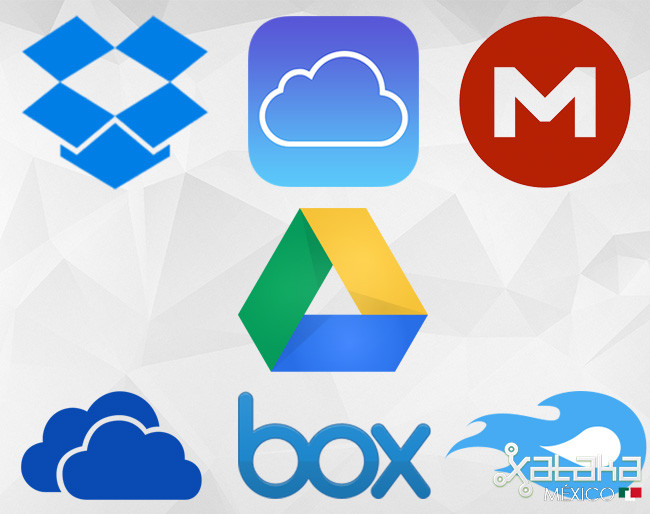
\includegraphics[width=7cm, height=4cm]{./images/servicios_nube.jpg}
\caption{Servicios de almacenamiento en la nube}
\label{fig:3-1-0}
\end{figure}


Ahora bien, si los clientes cifran convencionalmente sus archivos es decir usando la criptografía estándar (Simétrica y Asimétrica), se pierde ese ahorro de espacio. El cifrado convergente en adelante (\textit{CE}) resuelve esta problemática. Sin embargo, está inherentemente sujeto a ataques de fuerza bruta.\\

El protocolo criptográfico \textit{DupLESS} contiene una arquitectura que proporciona almacenamiento sin duplicados, seguro y resistente a ataques por fuerza bruta. En DupLESS, los clientes cifran sus archivos con claves basadas en mensajes, obtenidos
desde un servidor de llaves a través de una función llamada \textit{OPRF[(Oblivious Pseudorandom Function) Función Pseudoaleatoria de Poca Memoria] }. Esto permite a los clientes almacenar datos cifrados en na servicio de almacenamiento, y en este servicio se realiza la eliminación de archivos duplicados garantizando la confidencialidad del cliente. Dupless demuestra que el cifrado para el almacenamiento sin duplicados puede lograr ahorros de rendimiento y espacio ~\cite{dupless}. \\



%\textbf{Diseño} \\

%El protocolo criptográfico para la eliminación de duplicados DupLESS, está diseñado para proporcionar una solución para evitar ataques por fuerza bruta. En DupLESS, los usuarios cifran sus archivos con la ayuda de un servidor de claves en adelante \textit{(KS)} que está separado del servicio de almacenamiento en línea en adelante \textit{Nube}. Los usuarios se autentican en el $KS$, pero no pierden la información sobre sus datos. Mientras que el $KS$ permanezca inaccesible para los atacantes, el protocolo puede garantizar una alta seguridad de la información. Si en algún momento el $KS$ y la Nube están comprometidos, Dupless conserva la actual garantía $MLE[(Message Locked Encryption) Cifrado por Bloqueo de Mensaje]$ de seguridad para mensajes que no se pueden anunciar.\\ 

%Dupless está diseñado para implementarse de forma transparente con los sistemas en la Nube que hasta ahora se encuentran en funcionamiento como son Amazon, Dropbox, Google Drive, etc., por lo que DupLESS funciona como una capa sobre las interfaces de los sistemas en la Nube mencionados. Esto también significa que DupLESS pretende ser lo más compatible posible con los comandos existentes en las API's de estos sistemas en la Nube existentes, para que así Dupless no tenga ningún conocimiento sobre los sistemas que implementan estas API's, y logre dar un rendimiento muy cercano al de usar la Nube sin ningún cifrado obteniendo el mismo nivel de disponibilidad que hasta ahora estos sistemas proporcionan. \\


\textbf{Funcionamiento}\\

DupLESS contempla que un ataque por fuerza bruta a un texto cifrado dentro de un esquema de tipo CE puede tratarse utilizando un servidor de llaves $KS$ para derivar llaves a partir de un archivo, en lugar de establecer llaves con funciones hash de los archivos. Para poder acceder al $KS$, se debe de realizar el procedimiento de autenticación a los usuarios, esto detiene a los atacantes externos. El aumento de los costos a los ataques, disminuye los ataques por fuerza bruta hacia los usuarios.\\

%Para poder implementar un esquema seguro y que evite la duplicación de archivos, Dupless crea un servidor de llaves $KS$ el cuál proveerá de llaves para el cifrado de un archivo, dicho servidor se comunica con el cliente a través de un protocolo llamado $OPRF$, este protocolo proveerá de algoritmos para la autenticación de usuarios y el cifrado convergente de los archivos que se van a almacenar, dicho protocolo funciona de la siguiente manera: \\ 

DupLESS implementa un esquema que consta de cinco algoritmos (Kg, EvC, EvS, Vf, Ev), los últimos dos deterministas: 

\begin{itemize}
\item \textit{Generación de claves Kg: } \\

$(pk, sk) \stackrel{ \$ }{\longleftarrow} Kg$. 

Este algoritmo genera una llave pública \textit{pk= (e,n)} que puede distribuirse libremente entre varios usuarios, y una clave privada \textit{sk = (d,n)} que permanece sólo en el servidor de llaves. Estas llaves son generadas utilizando el algoritmo de RSA.

\item \textit{EvC: }\\ 
La evaluación de este protocolo comienza del lado del cliente: 
\begin {enumerate}
\item Se obtiene del servidor la clave pública \textit{e} y se realiza una comparación con \textit{e $\leq$ N}, $N$ fue el producto de 2 números primos utilizado en la generación de llaves del servidor. Si la comparación no se cumple, el protocolo envía un error.
\item Se elige un número aleatorio entero $r \stackrel{ \$ }{\longleftarrow} Z_{N}$.
\item Se realiza una función hash al archivo que se desea almacenar en Nube, es decir \textit{h ← H(M)} 
\item Ahora se multiplica la función hash del mensaje $M$ por el número aleatorio elevado a la llave pública del servidor (\textit{r$^e$}) y se almacena en \textbf{x}, es decir \textit{x ← h $\cdot$ r$^e$ $\bmod$ N}
\item Esta \textbf{x} es enviada al servidor de llaves, en donde será firmada por éste sin saber su contenido ni procedencia, es decir realizará una firma a ciegas del mensaje.
\item La firma realizada por el servidor es recibida en el cliente y se realiza la siguiente operación \hspace{2cm} \textit{z ← y $\cdot$ r$^{-1}$ $\bmod$ N} donde $z$ es la llave con la cual se cifrará el mensaje.


\end{enumerate}
\item \textit{EvS: }\\ 
Del lado del servidor, se recibe la entrada \textit{x} que corresponde al factor de ocultamiento del archivo enviada por el lado del cliente. El servidor sólo realiza una operación la cuál es la firma con la llave privada del servidor. Dicha firma es a ciegas ya que el servidor no conoce el contenido del archivo ni la procedencia de quien lo está enviando. Dicha firma se realiza de la siguiente manera: \hspace{2cm} \textit{y ← x$^d$ $\bmod$ N}


\item \textit{Vf: }\\

Este algoritmo de verificación se encarga de corroborar la firma realizada por el servidor, es decir, verifica que efectivamente sea el servidor de llaves $KS$ la entidad que realizó la firma a ciegas que el cliente estaba solicitando. Además, este algoritmo asegura que el archivo firmado por el servidor $KS$ sea el que el cliente envió. 
Dicho algoritmo opera de la siguiente manera: 
\begin{itemize}
\item Realiza la operación $z^e \bmod N $. Dicha operación se realiza para eliminar el factor de ocultamiento realizado por el cliente. De esta manera se puede llegar hasta la comprobación de la misma función hash generada en el cliente, si ésta es igual a la que estaba bajo el factor de ocultamiento, el algoritmo comprueba que el $KS$ firmó correctamente. 
\item Si el algoritmo realizó la operación \textit{z $^e$ $\bmod$ N} y el resultado en la comparación de las funciones hash no es el mismo, entonces el servidor no llevó a cabo correctamente el proceso de firmado y arroja un error. 

\end{itemize}

\item \textit{Ev: }\\
Como último algoritmo se encuentra $Ev$, dicho algoritmo se encarga del proceso de cifrado $C1$ del archivo original $M$ junto con la clave generada $z$ a través del proceso entre el cliente y el servidor $KS$. También realiza el cifrado $C2$ de la clave $z$ junto con la clave pública del usuario que desea almacenar un archivo. Dichas operaciones son las siguientes: 

\begin{itemize}
\item C1 ← $E_{z}(M)$
\item C2 ← $E_{pk}(z)$
\end{itemize}



\end{itemize}






